\section{The Blobs module}

Note: to avoid confusion, we refer the modules of the IPOL system as ``ipol modules'' and Python modules (files containing Python code) as ``Python modules''.

\subsection{Introduction}
Each demo of IPOL offers to the user a set of defaults blobs (\textbf{b}inary \textbf{l}arge \textbf{o}bjects). Thus, the users are not forced to supply their own files for the executions of the algorithms. These defaults blobs can be tagged and linked to differents demos.

The blobs module is composed of several Python modules. It is composed of the same technical stack as the rest of the rest of the IPOL modules: written in Python, using a web server, a database, and using templates for generating HTML responses for webservices destinated to humans.

\subsection{Main}
The main module is called by ``start.sh'', the script called by the control terminal to get modules running on different servers over ssh. It consist of setting up some variables used by cherrypy, as well as mounting the blobs class at the root of the used server.

\subsection{Error control}
This module describes the errors issued by the Blobs IPOL module and adds color to the error messages printed in the terminal.

\subsection{Databases}
The first and most important design constraint of the Blobs IPOL module was that data shouldn't be duplicated. All blobs referenced by multiple demos should exist in only one directory. This is addressed by establishment of one relational database, referencing the demos, the blobs, and the relationship between them. This database also permits to tag some text on blobs, as well as organize them in named sets. In the big picture, the database Python module a implement a simple CRUD\footnote{Acronym for Create, Read, Update, Delete. These operations allows the total manipulation and the persistence of data inside a data structure.} interface for manipulating the database. Blobs can be managed individually, and upon the deletion of a demo, the blobs related to this demo will be deleted from disk if and only if they were uniquely linked to this demo. Blobs are referenced via their hashes, making it easy to verify if a blob is already in the database, even under another filename. \\

\begin{figure}[h]
\centering
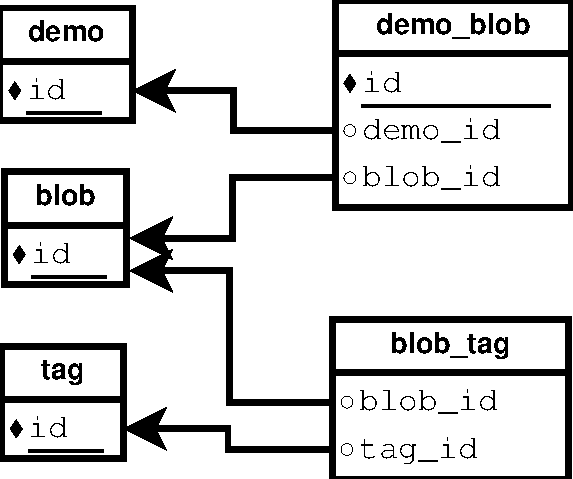
\includegraphics[scale=0.75]{blobs/images/blobs_database.pdf}
\caption{The database schema of the Blobs module.}
\label{fig:blobs_database}
\end{figure}

In the figure~\ref{fig:blobs_database}, id fields are the primary keys (it is worth noting that the primary key of a blob\_tag entry is the combination of the foreign keys it contains), the other fields are foreign keys, and the arrows indicate which primary keys are referenced by which foreign keys.
Three tables, demo, blob and tag, contains the information about referenced demos, blobs, and tags relating to blobs. Two junction tables link this information together, referencing the blobs standards to a demo, and the tags owned by each blobs.

\subsubsection{Database access}
This module offers an interface for accessing the database. One object of the class Database should be instanciated for each operation modifying it. Even if it has function for connecting and closing, they should not be used as such, for flow control issues (for example, an exception leaving a connection open). A very simple abstraction, the DatabaseConnection class, is present in the blobs Python module for the task of managing the connection. It allow a scope-controlled connection to the database, ensuring that it will be closed no matter what once the execution flow leave the scope where it was open, even when an exception is thrown.

Otherwise, this Python module offers us simple methods for interacting with the database, or obtaining metrics of it, such as the total number of blobs. They generally return the information asked if such case apply. For the format of the responses and the different function, we refer the reader to the code of the module itself. It is worth noting that one webservice, delete\_blob\_from\_demo, recompute the positions of the blobs in a set in which a blob was deleted. If this function is accessed concurrently by multiple threads (the most likely case is if a webservice calling this function is accessed several times in a very short span), the blobs can end up with miscalculated positions. Non-concurrential access should be enforced by locking the scope where this webservice is called. Such a lock is used in the delete\_blob\_ws webservice in the blobs Python module.

\subsection{The Blobs module}
The blobs Python module is the core of this. It implement three classes, DatabaseConnection as referenced earlier in the present documentation, and MyFieldStorage, for intermediate storage of the uploaded blobs in the /tmp/ directory, and Blobs as an encapsulation of the webservices and the data they use. It also has some utilitary function.

The Blobs class implements all the webservices constituting this module, as well as web pages generated via HTML templates. An instance of the Blobs class should possess information about the storage of blobs and the networking parameters cherrypy use, such as a port number. A cherrypy configuration file, named ``blobs.conf'' contains the informations one might need to change to run the module on another server, without changing the code, such as the directories where the blobs can be found, the port used by the cherrypy engine, or the path to the database.

The webservices of the module access the database via instanciations of Database objects managed by the DatabaseConnection class. Some read information, and some modify the database by adding or removing information. For handling a webservice automatically and charging his JSON response as a Python object, the utilitary function use\_web\_service is used.

Logging is utilized as a mean to retrieve the errors occuring in the system. The logger implemented in the blobs Python module handle all the errors of the module. It is passed to each Database object instanciation.

\subsection{Visual Representations}
Each blob is associated with a thumbnail that is used by the web interface to represent it (see figure~\ref{fig:blob_thumbnail_example}). This thumbnail is created during the upload of the blob.  

However, it is not possible to have a thumbnail for each possible blob, since they can not be visualized directly as in the case of hyperspectral images. In these cases, the representation of the blob would appear as broken in the web interface (see figure~\ref{fig:broken_representation}). For instance, the blobsets of an optical flow demo use a pair of consecutive images along with an optional ground-truth. This ground-truth is not an image and thus it is not possible to generate directly a thumbnail from it.
%

\begin{figure}[h]
\centering
\tcbox[sharp corners, boxsep=0.0mm, boxrule=0.1mm, colback=white]{
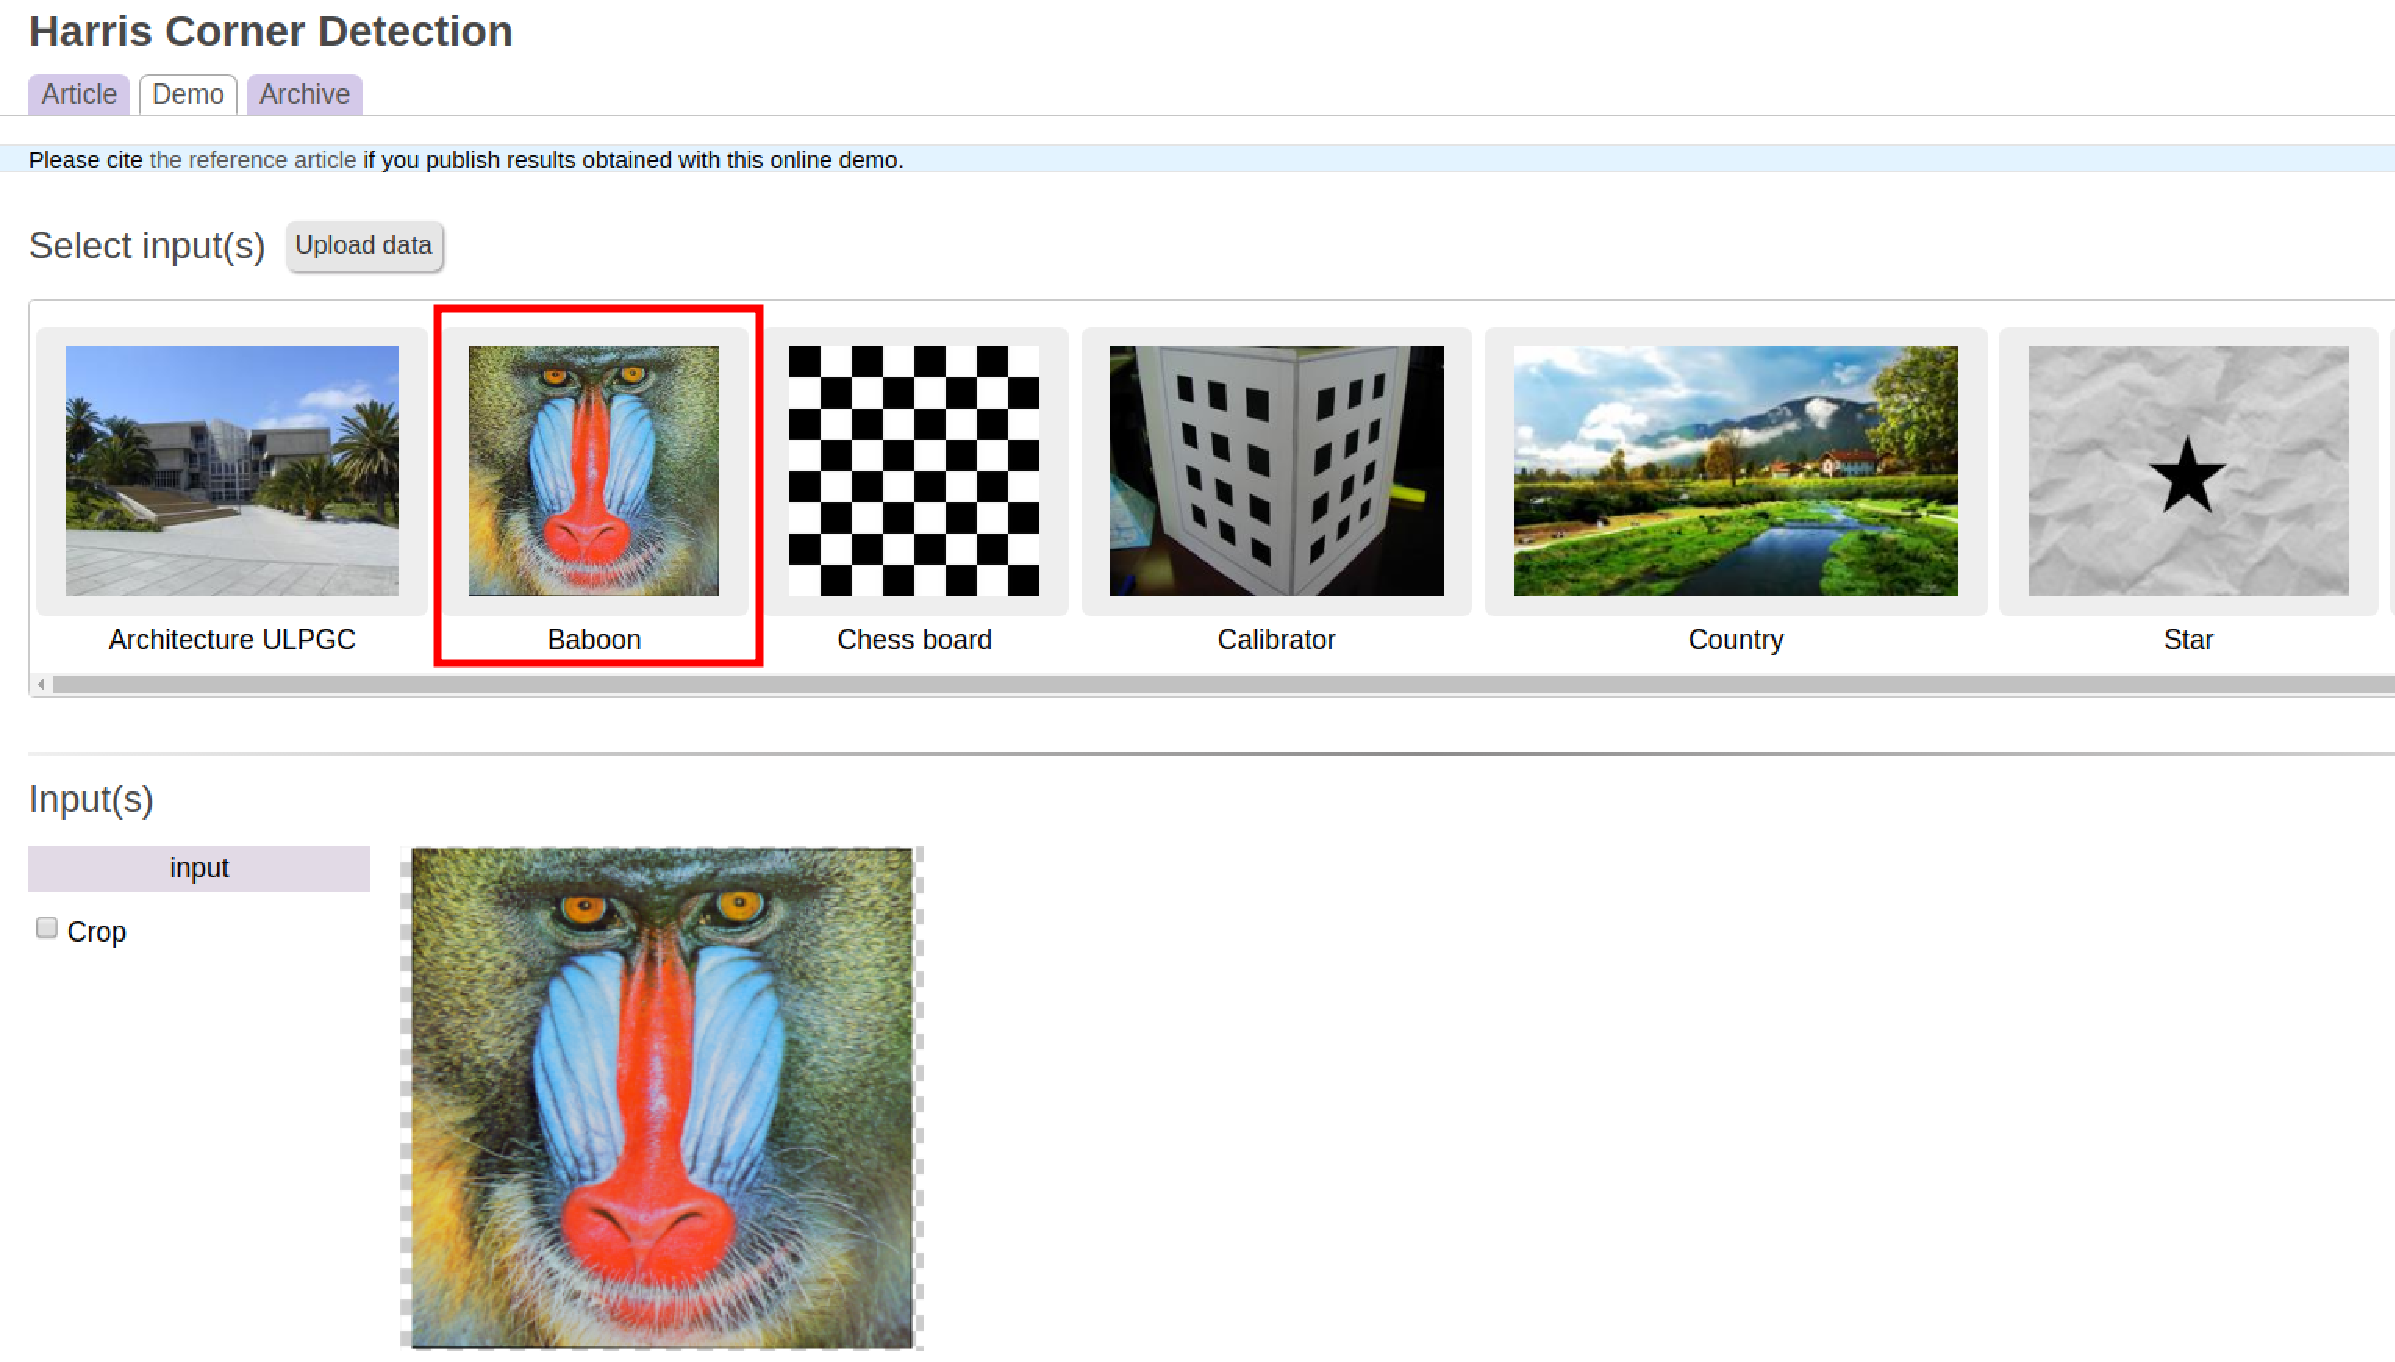
\includegraphics[scale=0.25]{blobs/images/blob_thumbnail_example.pdf}
}
\caption{Example of a blob representation using its thumbnail. In this example, the user has selected the Baboon image by pressing its corresponding thumbnail.} 
\label{fig:blob_thumbnail_example}
\end{figure}
%
\begin{figure}[h]
\centering
\tcbox[sharp corners, boxsep=0.0mm, boxrule=0.1mm, colback=white]{
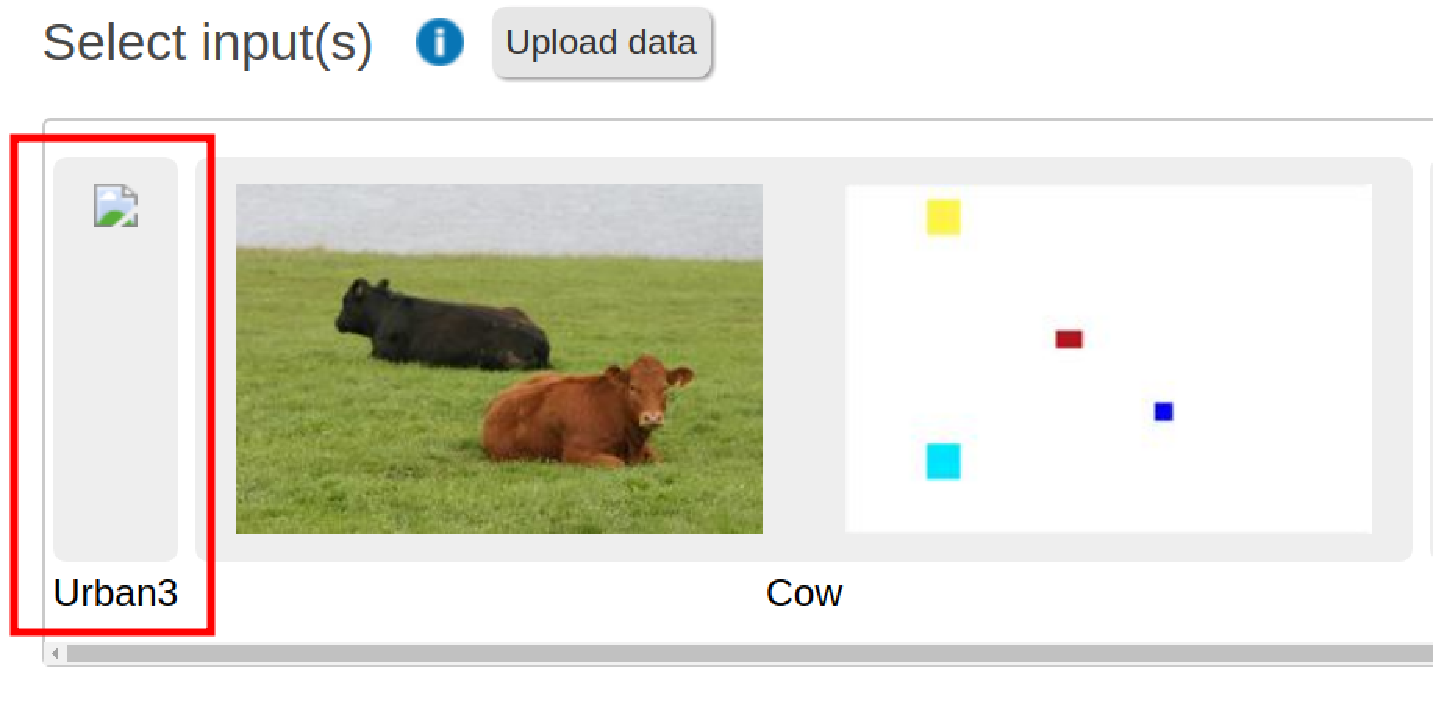
\includegraphics[scale=0.25]{blobs/images/broken_representation.pdf}
}
\caption{Broken image due to a blob that cannot be represented by the web interface.} 
\label{fig:broken_representation}
\end{figure}

A demo editor can avoid this situation by uploading an image as the visual representation the blob. The Blobs module stores the Visual Representation and creates the thumbnail from it. If the original blob already has a thumbnail the system overwrites it. Finally, the blob does not appear as broken in the web interface, as can be seen in figure~\ref{fig:visual_representation}.
%
\begin{figure}[h]
\centering
\tcbox[sharp corners, boxsep=0.0mm, boxrule=0.1mm, colback=white]{
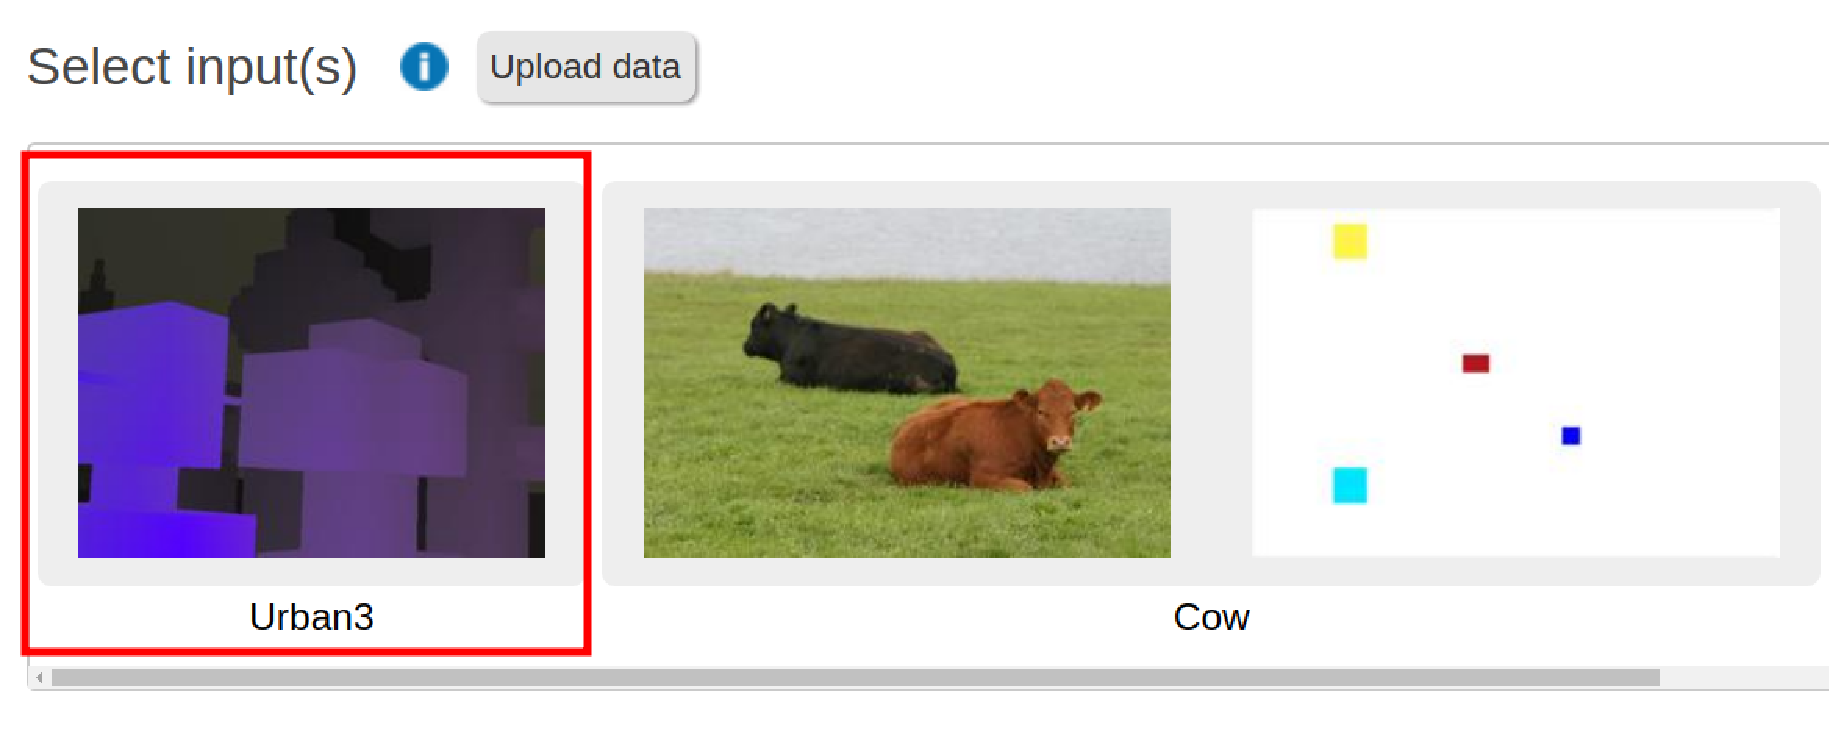
\includegraphics[scale=0.25]{blobs/images/visual_representation.pdf}
}
\caption{A visual representation has been uploaded for the blob in figure~\ref{fig:broken_representation}. The blob does not appear as broken in the web interface any more.} 
\label{fig:visual_representation}
\end{figure}
%


